\chapter{Testování}
Tato kapitola se zabývá testováním implemetovaného řešení nasazeného v produkčním prostředí. V první fázi je otestována stabilita řešení při velké zátěži a ve druhé uživatelská přívětivost procesu přidání zařízení a samotného webového rozhraní. Produkční prostředí běží ve virtualizovaném serveru se systémem Debian (linux), přidělenými hardwarovými prostředky: CPU (5 vláken Ryzen 3600), 9~GB RAM, HDD (7200 otáček). Použitá verze NodeJS 12.22.1, MongoDB 4.2.13 a RabbitMQ 3.8.14.

\section{Zátěžové testování}
Rozumně simulovat zátěž reálnými zařízeními lze pouze v jednotkách kusů, což s dnešním výkoným hardwarem není absolutně žádný problém obsloužit. Potřebuji však ověřit jak se systém bude chovat pod opravdovou zátěží - desítky paralelních požadavků a stovky připojených zařízení. Vytvořil jsem tedy automatizovaný test, kterému se definuje počet uživatelů a počet zařízení, které mezi uživatele má rozprostřít a o vše ostatní se test postará sám (pomocí HTTP požadavků stejně jako by uživatel interagoval přes webové rozhraní).

Prvně je vytvořen příslušný počet uživatelů a všechna virtuální zařízení (komunikující přes MQTT protokol stejně jako reálná). Všem uživatelům jsou načtena objevená zařízení, která jsou následně spárovaná a žačnou odesílát data ze senzorů a jiných vlastností simulující reálný provoz. Data se odesílají v náhodném rozmezí 50 - 60 vteřin, aby se provoz rozložil v čase. Test probíhal v následující konfiguraci:
\begin{itemize}
    \item počet uživatelů 25
    \item počet zařízení 250
    \item konfigurace zařízení - 2 senzory (teplota, vlhkost) a přepínač, data ze všech tří vlastností jsou odesíláná paralelně
    \item počet paralelních API požadavků 10
\end{itemize}
Pro sledování zátěže databáze byl využit \uv{Free monitoring} \cite{free-monitoring}, který sleduje dobu provádění operací, jejich počet a vytížení disku. Pro sledování zátěze cpu jednotlivých procesů byl použit linuxový nástroj \textit{htop} a pro vykreslení grafu celkové zátěže cpu \textit{Kibana}. Protože se jedná o více jádrový stroj, tak vytížení cpu nemá maximum 100\,\% ale pro každé jádro 100\,\% tedy celkem 500\,\%. Test byl proveden celkově 3x pro ověření správnosti naměřených dat. Tabulka dat, ze kterých byl sestaven graf na obrázku \ref{cpu-usage} je umístěna na přiloženém médiu viz. příloha \ref{medium}.

\begin{figure}[htbp]
    \centering
    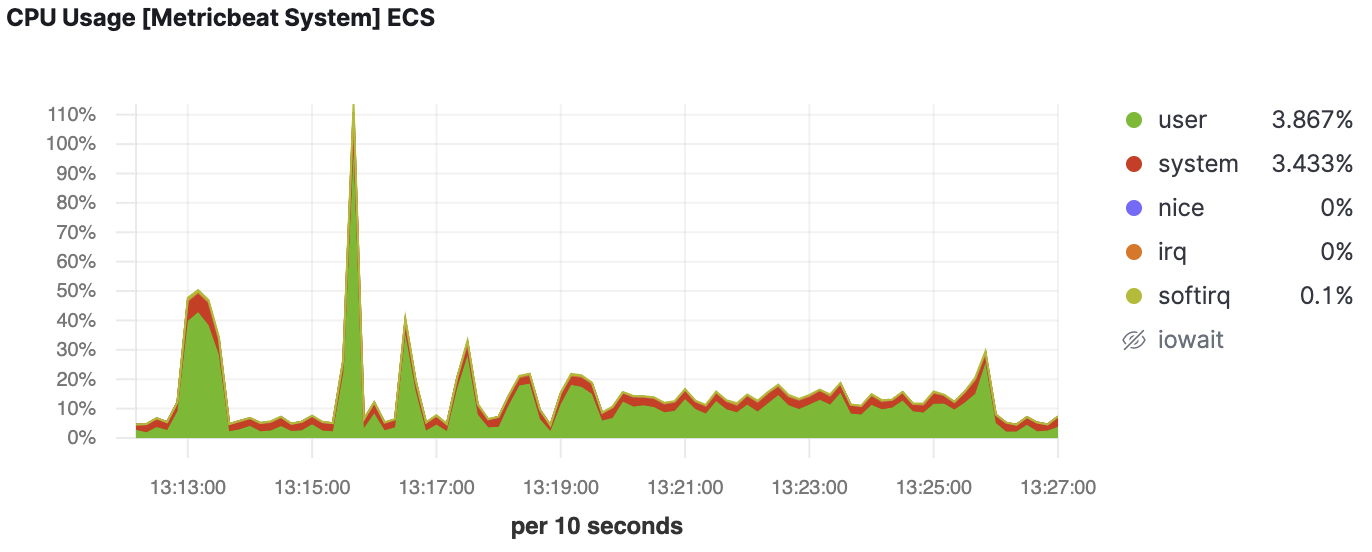
\includegraphics[width=\textwidth]{img/cpu_usage.png}
    \caption{\label{cpu-usage}Zátěž CPU během testu}
\end{figure}

První zvýšení trvající minutu je způsobeno zařízeními ohlašovujícími svoje vlastnosti, což způsobilo velký počet zápisů do databáze. Druhé zvýšení ve 13:15:40 trvající 20 vteřin způsobilo přidání jednotlivých zařízení uživatelům (a jejich spárování). Následující 10 min trvající zatížení bylo způsobeno tím, že zařízení odesílájí data ze svých vlasností. Závěrečná několika vteřinová zvýšená zátěž ve 13:25:50 je dána odesláním informace o odpojení ze všech zařízení. V průběhu testu byla průměrná doba vyřízení databázové operace 0,24 ms, zátěž cpu databází 8 \%, procesem Platformy 6 \% a zátěž disku přibližně 2 \%. V průběhu celého testu byla Platforma aktivně využívána uživatelem přes webové rozhraní k ovládání fyzických zařízení a po celou dobu vše reagovalo ihned bez jakéhokoliv zpoždění, ani průměrná doba zpracování RESTful požadavku nebyla významně ovlivněna. Z výsledku testu tedy vyplývá, že Platforma zvládne bez jakýhkoli problému obsloužit stovky zařízení bez negativního dopadu na výkon.


% popsat které části jsou náročné na DB maybe? Kolik DB query bylo během testu, čím jsem monitoroval prostředky, query max time, cpu usage

% protože se jedná o více jádrový stroj, tak % vytížení nemají max 100% ale 500%, protože 5 jader
% začátek - velký nápor trvající 1min, cpu až 100%, IOWait 80%, disk up to 60%
% průběh posílání dat - cpu - mongo 6%, node 6%
%                       - disk 1,5%
% za celou dobu doba provedení operace DB avg 0.12 ms, maximum 180 doc updated za sec, 
% v průběhu jsem používal Platformu a ovládal fyzická zařízení, která reagovala ihned a doba provedení api requestů byla stejná jako bez zatížení
% provedeny byly 3 testy s rozmezím 1 hodina, aby se minimalizoval případný dopad cachen na výkon

% z testy je vidět největší zátěž první minutu, kdy zařízení paralelně ohlašují svoje vlastnosti, následná dlouhodobá zátěž je způsobena neustálým odesíláním naměřených dat ze všech zařízení.

% \section{Zotavení po nenadálé události}

\section{Uživatelské testování}
Za pomoci uživatelského testování byla ověřena intuitivnost uživatelského prostředí. Cílem bylo zjistit zda uživatelé zvládnou vykonat základní úkony bez pomoci a zjistit jejich náročnost.

Každý uživatel dostal uživatelskou příručku (příloha \ref{user-guide}), přístup k již naprogramovanému zařízení, které ovládalo led světla a měřilo teplotu, a nakonec seznam úkonů, které mají vykonat a zpětně je ohodnotit na stupnici od jedné do pěti (pět je nejhorší). Před testem bylo vždy zařízení uvedeno do výchozího stavu.


\begin{figure}
    \centering
    % \begin{adjustbox}{angle=-90}
    % \begin{center} % pro addony přidat poznámku 324 obsahuje 2585 věcí
    \begin{tabular}{ | l | c | }
        \hline
        Úkon                           & Hodnocení \\
        \hline
        Připojte nové zařízení         & 3         \\
        \hline
        Zapněte led světla             & 1         \\
        \hline
        Podívejte se na průběh teplotu & 2         \\
        \hline
        Změňte umístění zařízení       & 1         \\
        \hline
        Zařízení odstraňte             & 1         \\
        \hline
    \end{tabular}
    \caption{Hodnocení jednotlivých testerů}
\end{figure}

V průběhu testování se ukázal jako nejvíce problematický první krok, ve kterém uživatel zadává v kaptivním portále údaje k připojení na domácí wifi a své uživatelské jméno k Platformě. Zařízení občas ohlásilo chybu připojení k wifi i při správně zadaných údajích. Po bližším zkoumání byl zjišten problém s knihovnoou \textit{WifiManager}, která má nastarosti vytvoření kaptivního portálu a následné připojení na wifi. Aktuální verzi této knihovny prochází rapidním vývojem s nedostatečnou dokumentací aktuálních funkcní. Nepodařilo se identifikovat jestli je problém se špatným využitím této knihovny či v implementaci knihovny samotné. Ostatní částí testu již probíhaly bez jakýhkoliv problému. Dle závěrečného hodnocení se rozhraní ukázalo jako uživatelsky velmi přívětivé a zařízení po prvotním úspěšném připojení k wifi pracovalo již naprosto spolehlivě.